\documentclass{article}
\usepackage[utf8]{inputenc}

% Version, bitte bei jeder Veröffentlichung entsprechend inkrementieren.
\newcommand{\version}{0.2.2}

% REMOVE THIS IF YOU WANT TO HAVE LINE INDENTS!!!
\setlength{\parindent}{0cm}

%\usepackage{fontspec}
%\setmainfont{[MyFont.ttf]}
%\setsansfont{[MyFont.ttf]} 

% Sonderzeichen ermöglichen
\usepackage[ngerman]{babel}
\usepackage[utf8]{inputenc}
\usepackage[T1]{fontenc}
\usepackage{a4wide}
\usepackage{xcolor}

% Section-Font
% \usepackage{sectsty}
% \sectionfont{\scshape}

\usepackage{bbm}
\usepackage{enumitem}
\usepackage{subfiles}
\usepackage{mathrsfs}
\usepackage{graphicx}
%
\usepackage{imakeidx}
\usepackage{hyperref}
%
\usepackage{graphicx}
\usepackage{tabularx}
\usepackage{booktabs} % Tabellen


\definecolor{javaKeyword}{RGB}{171, 35, 27}
\definecolor{javaComment}{RGB}{133, 133, 133}

\newcommand{\javaKeyword}[1]{\texttt{\textbf{\textcolor{javaKeyword}{#1\hphantom{.}}}}}

\newcommand{\javaIf}    {\javaKeyword{if}}
\newcommand{\javaElse}  {\javaKeyword{else}}
\newcommand{\javaFor}   {\javaKeyword{for}}
\newcommand{\javaWhile} {\javaKeyword{while}}
\newcommand{\javaDo}    {\javaKeyword{do}}
\newcommand{\javaNew}   {\javaKeyword{new}}
\newcommand{\javaThrow} {\javaKeyword{throw}}
\newcommand{\javaThrows}{\javaKeyword{throws}}
\newcommand{\javaClass} {\javaKeyword{class}}
\newcommand{\javaVoid}  {\javaKeyword{void}}
\newcommand{\javaInt}   {\javaKeyword{int}}
\newcommand{\javaLong}  {\javaKeyword{long}}
\newcommand{\javaByte}  {\javaKeyword{byte}}
\newcommand{\javaShort} {\javaKeyword{short}}
\newcommand{\javaChar}  {\javaKeyword{char}}
\newcommand{\javaFloat} {\javaKeyword{float}}
\newcommand{\javaDouble}{\javaKeyword{double}}
\newcommand{\javaVar}   {\javaKeyword{var}}
\newcommand{\javaInstanceof}    {\javaKeyword{instanceof}}
\newcommand{\javaPublic}        {\javaKeyword{public}}
\newcommand{\javaPrivate}       {\javaKeyword{private}}
\newcommand{\javaProtected}     {\javaKeyword{protected}}
\newcommand{\javaStatic}        {\javaKeyword{static}}

% New ones, TODO: add them to J2L
\newcommand{\javaTry}{\javaKeyword{try}}
\newcommand{\javaCatch}{\javaKeyword{catch}}
\newcommand{\javaSwitch}{\javaKeyword{switch}}
\newcommand{\javaCase}{\javaKeyword{case}}
\newcommand{\javaBreak}{\javaKeyword{break}}
\newcommand{\javaReturn}{\javaKeyword{return}}

\newcommand{\javaDoc}[1]{\textcolor{ForestGreen}{#1}}
\newcommand{\javaComment}[1]{\textcolor{javaComment}{#1}}
\newcommand{\javaDocAuthor}{\textbf{@author \hphantom{.}}}
\newcommand{\javaDocVersion}{\textbf{@version \hphantom{.}}}
\newcommand{\javaDocSee}{\textbf{@see \hphantom{.}}}
\newcommand{\javaDocParam}{\textbf{@param \hphantom{.}}}


\newcommand{\codemarkup}[1]{\texttt{#1}}
\newenvironment{code}{\ttfamily}{}

\makeindex[title=Definitionsübersicht, columns=2, intoc]
%\usepackage{sourceserifpro}

%\usepackage{wrapfig}
%\usepackage{caption}
%\captionsetup[wrapfigure]{margin=0cm, textfont=small, labelfont=small}

%\usepackage{graphicx}
%\graphicspath{ {./images/} }

% Font-awesome
%\usepackage{fontspec}
\usepackage{fontawesome}

%Bilder
\graphicspath{ {./images/}}

\setcounter{tocdepth}{4}
\setcounter{secnumdepth}{4}

% Author-Information
%\newcommand{\ushortWithMail}[1]{\href{mailto:#1@student.kit.edu}{#1}}
\newcommand{\ourMails}[1]{\href{mailto:uwgmn@student.kit.edu;ujict@student.kit.edu;uzytw@student.kit.edu;udlzq@student.kit.edu?subject=SWT-Zusammenfassung}{#1}}
\newcommand{\ushort}{\ourMails{uwgmn, ujict, uzytw, udlzq}}
\newcommand{\myName}{Julian Keck, Julian Leitner, Christian Schliz, Niklas Seng}
\newcommand{\myEmail}{\ushort@student.kit.edu}
\newcommand{\creationYear}{2021}

\newcommand{\figA}[2]{
    \begin{figure}[h]
        \centering
        \includegraphics[width=1\textwidth]{#2}
        \caption{#1}
    \end{figure}
}
\usepackage{caption}
\newcommand{\fig}[2]{
    % \newline
    %\hspace{\dimexpr-\fboxrule-\fboxsep\relax}\fbox
}

%Kopf und Fußzeile
%\usepackage{scrlayer-scrpage}
%\pagestyle{scrheadings}
%\ihead{}
%\chead{}
%\ohead{}
%\lofoot{\ourMails{\footnotesize Fehler oder Vorschläge? $\Rightarrow$ Schreib gerne ne Mail \faEnvelope }}
%\cfoot{\pagemark}
%\rofoot{\small{\faCopyright}  \ushort $\;$-$\;$\creationYear}
 %\pagemark

% Layout


%Subtitle
\usepackage{relsize}
\newcommand{\subtitlerelsize}{1} %relative size: integer value
\newcommand{\subtitlelinesep}{0.1em} %line separation: a LaTeX length

% Hyperlinks in das Dokument einfügen
\usepackage{hyperref}

% Mathe-Packages einbinden
\usepackage{amsmath}
\usepackage{amssymb}
\usepackage{amsthm}

% Graphen
\usepackage{tikz}
\usetikzlibrary{trees}

% Balken neben Texten
\usepackage[color, leftbars]{changebar}
\setlength\changebarsep{5pt}

% Aufzählingsbeschriftung anpassen
\renewcommand\labelenumi{(\roman{enumi})}
\renewcommand\theenumi\labelenumi

%Farbdefinitionen
\definecolor{strongColor}{RGB}{189, 66, 0}
\definecolor{lightblue}{RGB}{0, 140, 232}
\definecolor{importantColor}{RGB}{163, 19, 0}
\definecolor{ForestGreen}{RGB}{34,139,34}

% Mathematik-Definitionen
\newcommand{\N}{\mathbb{N_+}} %Natürliche Zahlen (ohne 0)
\newcommand{\Nz}{{\mathbb{N}_0}} %Natürliche Zahlen (mit 0)
\newcommand{\Z}{\mathbb{Z}} % Ganze Zahlen
\newcommand{\Q}{\mathbb{Q}} % Rationale Zahlen
\newcommand{\R}{\mathbb{R}} % Reelle Zahlen
\newcommand{\C}{\mathbb{C}} % Komplexe Zahlen
\newcommand{\K}{\mathbb{K}} % Körper
\newcommand{\F}{\mathbb{F}} % Fields [F_2]
\newcommand{\matr}[1]{\begin{pmatrix}#1\end{pmatrix}} % Matrizen [leider ist \matrix wegen asmmath nicht direkt möglich.]
\newcommand{\vektor}[1]{\matr{#1}} %Vektoren
\newcommand{\set}[1]{\{#1\}} % Mengen
\newcommand{\ematr}{\mathbbmtt{1}}
\newcommand{\invers}[1]{#1^{-1}}   % Inverse einer Zahl. Für x -> x^-1
\newcommand{\vectors}[1]{#1_1, \dots, #1_n}


%\newcommand{\todo}{\strong{TODO: }}
\newcommand{\todo}[1]{
    \PackageWarning{TODO}{#1}
    % \PackageError{TODO}{#1}
    %\textbf{\textsc{\textcolor{red}{TODO: #1}}}
}

\newcommand{\kapitel}[2]{Kapitel #1 - \textsc{#2}}

\newcommand{\emptyline}[0]{$\>$\\}
\newcommand{\n}[0]{$\>$\\}

% Farbdefinitionen
\newcommand{\blue}[1]{\textcolor{blue}{#1}}
\newcommand{\red}[1]{\textcolor{red}{#1}}
\newcommand{\babyblue}[1]{\textcolor{lightblue}{#1}}
\newcommand{\strongColor}[1]{\textcolor{strongColor}{#1}}

% Text-Layout-Spezifische commands!
\newcommand{\strong}[1]{\textbf{\strongColor{#1}}}
\newcommand{\important}[1]{\textcolor{importantColor}{#1}}

% Definitionen
%\newcommand{\definition}[3][1]{}
\newcommand{\definition}[3][1]{
    \noindent
    % TODO: fix minipage-padding to next definition
    \begin{minipage}{\linewidth}
    \faArchive$\:$
    \textbf{\textcolor{lightblue}{#2}}
    \cbstart
    %(\textit{#2})
    \cbcolor{lightblue}
    #3
    \cbend
    \newline
    \ifnum#1=1\break\else\textsc{}\fi
    % Stichwortverzeichnis am Ende erzeugen.
    \index{
        \vspace{0.2cm}
        \hspace*{-0.5cm}
        \underline{\textsc{#2}}\\
        #3
    }
    \end{minipage}
}

% Definitionen
\newcommand{\principle}[3][1]{
    \noindent
    \faExclamationCircle$\:$
    \textbf{\textcolor{orange}{#2}}
    \cbstart
    %(\textit{#2})
    \cbcolor{orange}
    #3
    \cbend
    \newline
    \ifnum#1=1 \break\else\textsc{}\fi
    %
}

\newcommand{\warn}[3][1]{
    \principle[#1]{#2}{#3}
}

% Definitionen
\newcommand{\imp}[3][1]{
    \noindent
    \faExclamationCircle$\:$
    \textbf{\textcolor{red}{#2}}
    \cbstart
    %(\textit{#2})
    \cbcolor{red}
    #3
    \cbend
    \newline
    \ifnum#1=1 \break\else\textsc{}\fi
    %
}

% Anmerkung
\newcommand{\anmerkung}[3][1]{
    \noindent
    \faLightbulbO$\:$
    \textbf{\textcolor{ForestGreen}{#2}}
    \cbstart
    %(\textit{#2})
    \cbcolor{ForestGreen}#3
    \cbend
    \newline
    \ifnum#1=1 \break\else\textsc{}\fi
}



\newcommand{\verweis}[1]{\textcolor{ForestGreen}{#1}}
\newcommand{\example}[1]{\textit{Beispiel: }#1}
\newcommand{\anfuehrung}[1]{\flqq #1\frqq}

\newcommand{\abb}[3]{#1:\;\begin{aligned}[t]#2\\#3\end{aligned}}





\title{SWT1 – kondensiertes Modulskript im SS 2021\\[\subtitlelinesep]%
    \smaller[\subtitlerelsize]{}Version \version}
\author{\ushort\\\myName}

\date{Stand: \today}



\begin{document}
%\maketitle
%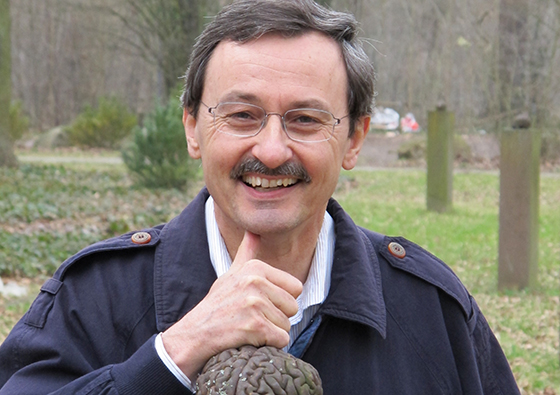
\includegraphics[width=\textwidth]{./data/tichy}
% \href{https://www.youtube.com/watch?v=q7oVvnlR0oQ}{\includegraphics[width=\textwidth]{spaltendermatrix}}
%\newpage

%\tableofcontents
%\newpage

\section{GIT}
% Bild 1
\fig{Lebenszyklus einer Datei in Git}{./data/git_lebenszyklus}
% Bild 2
\fig{Remote-Repository \& Local-Respoitory}{./data/git_remote_local}

\section{Sichtbarkeiten in Java}
\fig{Sichtbarkeiten in Java}{./data/javasichtbarkeit}
% Taken from: https://stackoverflow.com/questions/215497/what-is-the-difference-between-public-protected-package-private-and-private-in
\section{Lastenheft}
\definition[0]{Lastenheft}{Das Lastenheft beschreibt das System in der Sprache des Kunden. Insbesondere soll also der Kunde einen Überblick erhalten.}
\subsubsection{Bestandteile}
\begin{itemize}
    \item Zielbestimmung
    \item Produkteinsatz/Zweck/Zielgruppe/Plattform
    \item Funktionale Anforderungen
    \item Produktdaten (welche Daten werden gespeichert?)
    \item Nichtfunktionale Anforderungen
    \item Systemmodelle (Szenarien, Anwendungsfälle)
    \item Glossar (Lexikon zu Produktbeschreibungen)
\end{itemize}
\section{Pflichtenheft}
\subsection{Modellierung}
Das Pflichtenheft liefert ein Modell des zu implementierenden Systems.\\
Modell-Arten:
\begin{itemize}
    \item \important{Funktionales} Modell (aus dem Lastenheft)
    \begin{itemize}
        \item Szenarien und Anwendungsfall-Diagramme
    \end{itemize}
    \item \important{Objektmodell}
    \begin{itemize}
        \item Klassen- und Objektdiagramme
    \end{itemize}
    \item \important{Dynamisches} Modell
    \begin{itemize}
        \item Sequenzdiagramme
        \item Zustandsdiagramme
        \item Aktivitätsdiagramme
    \end{itemize}
\end{itemize}

\newpage

\section{Entwurfsmuster - Kategorien}
\begin{table}[h]
\begin{tabular}{l|l}
\toprule
Kategorie & Muster   \\\midrule
Entkopplungsmuster & Adapter, Beobachter, Brücke, Iterator, Stellvertreter, Vermittler  \\\hline
Variantenmuster & Abstrakte Fabrik, Besucher, Fabrikmethode, Kompositum, \\& Schablonenmethode, Strategie, Dekorierer \\\hline
Zustandshandhabungsmuster & Einzelstück, Fliegengewicht, Memento, Prototyp, Zustand  \\\hline
Steuerungsmuster & Befehl, Master/Slave (Master/Worker)  \\\hline
Virtuelle Maschinen &   \\\hline
Bequemlichkeitsmuster & Bequemlichkeitsklasse, Bequemlichkeitsmethode, Fassade, Null-Objekt \\\bottomrule
\end{tabular}
\end{table}

\section{Bewertung von parallelen Algorithmen}
\subsection{Gesamtlaufzeit}
\[
    \mathcal{T}(p) = \sigma + \frac{\pi}{p}, \text{ wobei}
\]
 $\sigma$ die Zeit für die Ausführung des sequentiellen Teils und\\
 $\pi$ die Zeit für die sequentielle Ausführung des parallelisierbaren Teils darstellt.
 
 \subsection{Beschleunigung (\textit{Speedup})}
 \[
    \mathcal{S}(p)=\frac{\mathcal{T}(1)}{\mathcal{T}(p)}
 \]
 \subsection{Effizienz}
 \[
    \mathcal{E}(p) = \frac{\mathcal{T}(1)}{p\cdot \mathcal{T}(p)} = \frac{\mathcal{S}(p)}{p}
 \]
 Idealfall:\\
 $\Rightarrow$ $\mathcal{S}(p)=p$ und $\mathcal{E}(p)=1$

\section{Testen} 
\fig{Pfadüberdeckungsbeispiel}{./data/pfazeigüberd}
\definition[0]{Die Pfadüberdeckung}{fordert die Ausführung aller unterschiedlichen, vollständigen Pfade im Programm.}
\begin{itemize}
    \item Anweisungsüberdeckung
    $A = \{(Start,1,2,3,4,5,Stopp)\}$
    \item Zeigüberdeckung
    $Z = A \cup \{(Start,1,3,5,Stopp)\}$
    \item Pfadüberdeckung
    $P = Z \cup \{(Start,1,3,4,5,Stopp)\} \cup \{(Start,1,2,3,5, Stopp)\}$
\end{itemize}

\section{Teufelsquadrat in der Softwareplanung}
\fig{Teufelsquadrat mit beispielhafter Erhöhung der Qualität und Entwicklungsdauer sowie der resultierender Erhöhung der Kosten und geminderter Quantität}{./data/Teufelsquadrat.png}

\section{COCOMO-II - Formel}
\[PM=A \cdot (Size)^{1,01+0,01 \cdot \sum^{5}_{j=1}SF_j} \cdot \prod^{17}_{i=1}EM_i\]


%\newpage

%\printindex
%\newpage
%\listoffigures
\end{document}